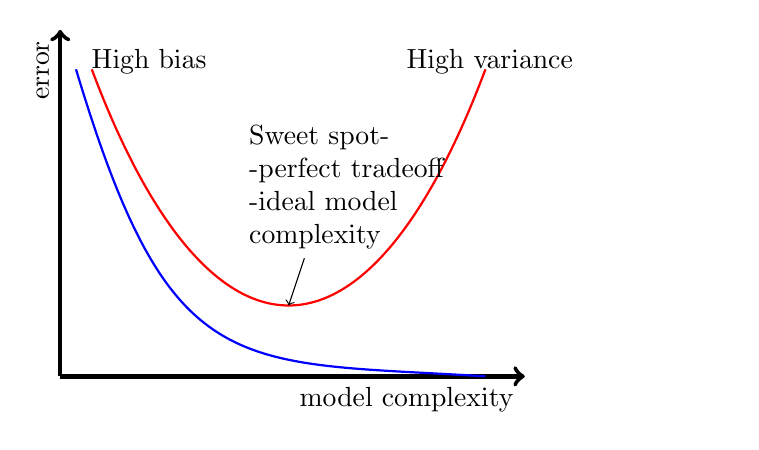
\begin{tikzpicture}
	\draw[->,ultra thick] (4.1,-0.9)--(10,-0.9) node[below left]{model complexity};
	\draw[->,ultra thick] (4.1,-0.9)--(4.1	,3.5) node[above left,rotate=90]{error};
					
	\onslide<5->{\draw[red,thick] (4.5,3) .. controls (6,-1) and (8,-1) .. (9.5,3);}
	\onslide<6->{\draw[blue,thick] (4.3,3) .. controls (5.5,-1) and (6.3,-0.7) .. (9.5,-0.9);}
	\onslide<7->{\node[text width=4cm] at (6.5,3.1) {High bias};}
	\onslide<8->{\node[text width=4cm] at (10.5,3.1) {High variance};}
	\onslide<9->{\node[text width=3cm] at (8,1.5) {Sweet spot-\\-perfect tradeoff \\ -ideal model\\ complexity};}
	\onslide<9->{\draw[->] (7.2,0.6)--(7,0);}			
\end{tikzpicture}